\documentclass{article}
\usepackage{graphicx}
%\usepackage[a4paper]{geometry}
\usepackage{fullpage}
\usepackage{listings}
\usepackage{color}
\setcounter{secnumdepth}{5}
\lstset{
basicstyle=\ttfamily,
language=C++,
frame=single,
tabsize=2,
keywordstyle=\color{blue},
stringstyle=\color{mauve},
breaklines=true,
escapeinside={\%*}{*},
showspaces=false,
showstringspaces=false
}


\begin{document}
\title{Compositional Dataflow}
\date{}
\maketitle
\section{Abstract Object Interface}
\noindent
The abstract object is a basic abstraction for symbolic values and
memory locations implemented by the compositional dataflow framework. The
AbstractObject has three main sub-classes. 
\begin{itemize}
\item MemLocObject 
\item ValueObject 
\item CodeLocObject
\end{itemize}
The AbstractObject interface requires two main functionalities to be
implemented by its derived objects.
\begin{lstlisting}
bool  mayEqual(AbstractObjectPtr, PartEdgePtr)
bool mustEqual(AbstractObjectPtr, PartEdgePtr)
\end{lstlisting}
\emph{source files: abstract\_object.h, abstract\_object.C}
\subsection{MemLocObject}
MemLocObject is an abstraction for memory locations. The memory
objects have two ways of classifying them. 
\subsubsection{Classification based on Memory Organization}
The first is using the
memory organization to described them.
\begin{description}
\item Scalar: \emph{no memory organization}
\item LabeledAggregate: \emph{struct/class}
\item Pointer: \emph{objects that may point to others}
\item Array: \emph{contiguous sequences of memory objects}
\end{description}
\subsubsection{Classification based on Syntactic Information}
The second classification is based on syntactic information. In this
classification the type is used to determine the nature of the
object. This classification is implemented by StxMemLocObect.
 It is roughly classified into three categories.
\begin{description}
\item NamedObj: \emph{memory objects for variable declarations}
\item ExprObj:\emph{memory objects for temporary expressions}
\item AliasedObj: \emph{memory objects for objects pointed to by pointers}
\end{description}
Combining the two classifications, the memory objects can be any of
the following.
\begin{enumerate}
\item ScalarNamedObj
\item ScalarExprObj
\item ScalarAliasedObj
\item LabeledAggregateNamedObj
\item LabeledAggregateExprObj
\item LabeledAggregateAliasedObj
\item ArrayNamedObj
\item ArrayExprObj
\item ArrayAliasedObj
\item PointerNamedObj
\item PointerExprObj
\item PointerAliasedObj
\end{enumerate}
The inheritance hierarchy for ScalarNamedObj is shown in Fig \ref{fig:sno_inherit_graph}
\begin{figure}[htb]
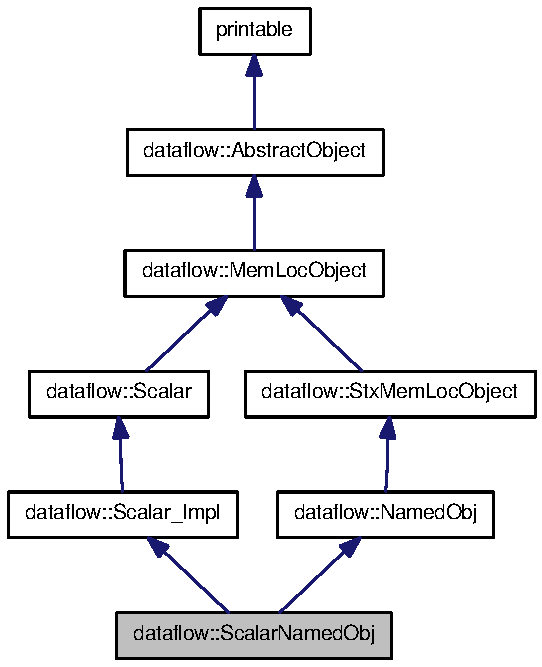
\includegraphics{sno-inherit-graph.pdf}
\caption{Inheritance hierarchy for ScalarNamedObj}
\label{fig:sno_inherit_graph}
\end{figure} \\
\subsubsection{Implementation of MemLocObject may/mustEquality}

MemLocObject requires its derived objects to implement the following
two methods. 
\begin{lstlisting}
virtual bool 	mayEqualML (MemLocObjectPtr o, PartEdgePtr pedge)=0
virtual bool 	mustEqualML (MemLocObjectPtr o, PartEdgePtr pedge)=0
\end{lstlisting}
On comparing may or mustEquality of two ExprObj, MemLocObject
uses the derived implementation of the two functions.
\begin{lstlisting}
 if((dynamic_cast<const ExprObj*>(this)  && dynamic_cast<const ExprObj*>(o.get())) ||
     (!dynamic_cast<const ExprObj*>(this) && !dynamic_cast<const ExprObj*>(o.get())))
  { return mayEqualML(o, pedge); }
\end{lstlisting}
\subsubsection{MemLocObjectPtrPair}
This class is a wrapper for MemLocObject.
\begin{lstlisting}
// Holds a pair of MemLocObjectPtr (one for the expression object and another for the object in memory) and provides 
// basic functionality to accessing them easily
class MemLocObjectPtrPair : public printable
{
public:
  // It is always true that one or both of expr and mem are non-null
  MemLocObjectPtr expr;
  MemLocObjectPtr mem;
\end{lstlisting}
The interactions between analyses happen using the
MemLocObjectPtrPair object i.e the
Composer always return \texttt{MemLocObjectPtrPair} for its
\texttt{Expr2MemLoc( )} method.\\
\large{TODO: list cases that requires both expr and mem to be not NULL}

\subsubsection{CombinedMemLocObject$<$defaultMayEq$>$}
This class maintains multiple MemLocObjects. The purpose of this class
is to maintain multiple memory abstractions about a particular object
and respond with least accurate (Union) or most accurate
(Intersection) answers to queries.
\begin{lstlisting}
template <bool defaultMayEq>
class CombinedMemLocObject : public virtual MemLocObject
{
  public:
  std::list<MemLocObjectPtr> memLocs;
..
};
typedef CombinedMemLocObject<false> IntersectMemLocObject;
typedef CombinedMemLocObject<true> UnionMemLocObject;
\end{lstlisting}
The CombinedMemLocObject is classified only based on the memory
organization. The different CombinedMemLocObjects are
\begin{itemize}
\item CombinedScalar
\item CombinedLabeledAggregate
\item CombinedArray
\item CombinedPointer
\end{itemize}
\begin{figure}[htb]
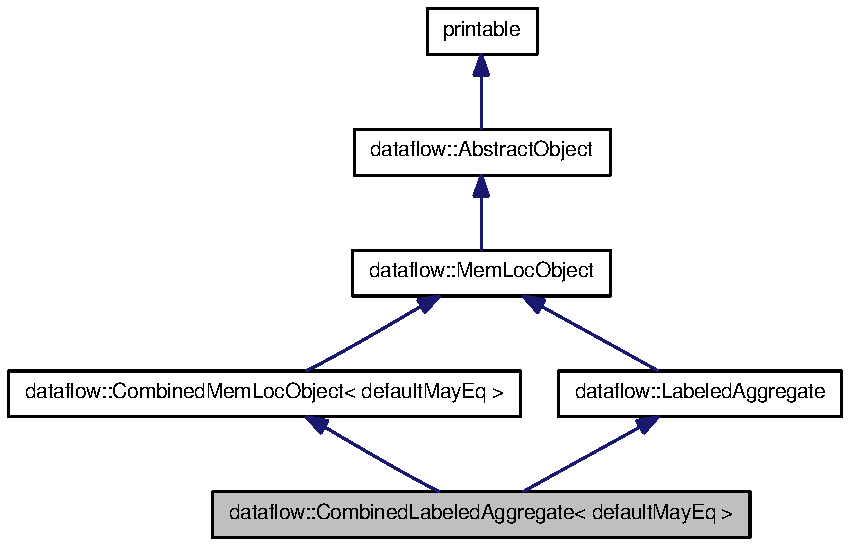
\includegraphics{cla-inherit-graph.pdf}
\caption{Inheritance hierarchy of CombinedLabeledAggregate}
\label{fig:cla_inherit_graph}
\end{figure}
The inheritance hierarchy of CombinedLabeledAggregate is shown in Fig \ref{fig:cla_inherit_graph}
\paragraph{Implementation of CombinedMemLocObject::create}
\paragraph{Implementation of CombinedMemLocObject::may/mustEqualML}

\subsubsection{Implementation of Pointer::getDereference()}


\subsection{ValueObject}
\subsection{CodeLocObject}

\section{Composer Interface}
The Composer serves as the intermediary between different analyses.  A
client analysis queries the composer and the composer responds by
returning appropriate abstract object from previously executed
analyses. For AbstractObjects, the Composer exposes the following functions.
\begin{lstlisting}
ValueObjectPtr Expr2Val(SgNode*, PartEdgePtr, ComposedAnalysis*)
ValueObjectPrt OperandExpr2Val(SgNode* n, SgNode* operand,
PartEdgePtr, ComposedAnalysis*)
\end{lstlisting}

\begin{lstlisting}
MemLocObjectPtrPair Expr2MemLoc(SgNode*, PartEdgePtr, ComposedAnalysis*)
MemLocObjectPtrPair OperandExpr2MemLoc(SgNode* n, SgNode* operand,
PartEdgePtr, ComposedAnalysis*)
\end{lstlisting}

\begin{lstlisting}
CodeLocObjectPtrPair Expr2CodeLoc(SgNode*, PartEdgePtr,
ComposedAnalysis*)
\end{lstlisting}

\begin{lstlisting}
PartPtr GetFunctionStartPart(const Function&, ComposedAnalysis*)
PartPtr GetFunctionEndPart(const Function&, ComposedAnalysis*)
\end{lstlisting}

\noindent ChainComposer implements the functionality of the composer.
\emph{sources: compose.h/compose.C}

\end{document}